\phantomsection
\chapter[Finding Motifs in Transcription Factor Networks]{Finding Motifs in Transcription Factor Networks\chapsubhead{Noah Lee and Phillip Compeau}}
\label{chapter:motifs}
\renewcommand{\chaptertitle}{Finding Motifs in Transcription Factor Networks}
\addcontentsline{cc}{chapter}{Chapter \thechapter} % Adds chapter number to table of contents


\FloatBarrier

\section{Networks Rule (Biology)}
\label{sec:introduction}
\phantomsection

In \autoref{chapter:turing}, we worked with a particle-based model that simulated the interactions of skin cells to produce complex Turing patterns. In this chapter, we will zoom into the molecular level and model protein interactions. The scale of these interactions is tiny: a protein is typically on the order of about 10nm in diameter. (For comparison, the diameter of a single human hair is about 100,000 nm, and a light microscope's highest resolution is about 2,000 nm.) We will see that the cell has evolved a form of molecular communication based on protein interactions that is rapid, robust, and elegant.

To model protein interactions, we will use a  \textdef{network}{network}{a collection of nodes, pairs of which are connected by one- or two-directional segments or arcs called edges}, which is a collection of \textdefnogloss{nodes} along with \textdefnogloss{edges} that connect pairs of nodes. Whether we are studying the interactions of proteins, the complex chains of chemical reactions underlying cellular metabolism, the tangled webs of neurons in the human nervous system, or an evolutionary tree of life, networks are critical to our understanding of biological processes.

Our interest lies in the frequently recurring structures hidden within biological networks called \textdef{network motifs}{network motif}{a recurring substructure in a network}. Similarly to our work in \autoref{chapter:turing}, we will use modeling to answer \textit{why} these motifs have evolved to help the cell respond to its environment.

We will soon define our specific network of study, but before we get ahead of ourselves, we will introduce some molecular biology fundamentals that we will need to complete our analysis. You may already know this biological background, in which case you should feel free to skim the next section.\\

\FloatBarrier
\phantomsection

\section{Transcription and DNA-Protein Binding}
\label{sec:transcription_and_dna-protein_binding}
\phantomsection

\subsection{The central dogma of molecular biology}

DNA is a double-stranded molecule consisting of the four nucleobases adenine, cytosine, guanine, and thymine; the sum total of a cell's DNA constitutes its \textdef{genome}{genome}{the total of a cell's DNA}. A \textdef{gene}{gene}{a sequence of DNA nucleotides that serves as a template for the production of RNA, which may then be translated into protein} is a region of an organism's DNA that is \textdef{transcribed}{transcription}{the process by which one strand of a double-stranded DNA molecule is used as a blueprint for the production of a single strand of RNA} into a single-stranded RNA molecule, in which thymine is converted to uracil and the other bases remain the same.

The RNA transcript is then \textdef{translated}{translation}{the process by which a single-stranded RNA molecule is used as a template for the production of a polypeptide chain of amino acids} into an amino acid sequence. Because there are four different bases but twenty amino acids available, RNA is translated in \textdef{codons}{codon}{a triplet of RNA nucleotides, which encodes a single amino acid during translation}, or triplets of nucleobases. \autoref{fig:central_dogma}(top) shows the way in which codons are translated into amino acids, which is called the \textdef{genetic code}{genetic code}{the set of rules according to which each of the 64 possible triplets of RNA nucleotides, called codons, are converted into one of the 20 standard amino acids (two codons do not correspond to any amino acid and are called stop codons, as they halt translation)}.

DNA can therefore be thought of as a blueprint for storing information that flows from DNA to RNA to protein. This flow of information is called the \textdef{central dogma of molecular biology}{central dogma of molecular biology}{the paradigm that genetic information in the cell flows from DNA to RNA via transcription and from RNA to protein via translation} and is illustrated in \autoref{fig:central_dogma} (bottom).\\

\begin{figure}[hp]
\centering
\mySfFamily
\tiny
\tabcolsep = 0.5em
\rowcolors{2}{gray!25}{white}
\begin{tabular}{c l@{\hspace{2.5em}} c l @{\hspace{2.5em}} c l @{\hspace{2.5em}} c l}
\rowcolor{gray!50}
\textbf{Codon} & \textbf{Amino acid} & \textbf{Codon} & \textbf{Amino acid} & \textbf{Codon} & \textbf{Amino acid} & \textbf{Codon} & \textbf{Amino acid}\\
\textnucl{AAA} & Lysine & \textnucl{AAC} & Asparagine & \textnucl{AAG} & Lysine & \textnucl{AAU} & Asparagine\\
\textnucl{ACA} & Threonine & \textnucl{ACC} & Threonine & \textnucl{ACG} & Threonine & \textnucl{ACU} & Threonine\\
\textnucl{AGA} & Arginine & \textnucl{AGC} & Serine & \textnucl{AGG} & Arginine & \textnucl{AGU} & Serine\\
\textnucl{AUA} & Isoleucine & \textnucl{AUC} & Isoleucine & \textnucl{AUG} & Methionine & \textnucl{AUU} & Isoleucine\\
\textnucl{CAA} & Glutamine & \textnucl{CAC} & Histidine & \textnucl{CAG} & Glutamine & \textnucl{CAU} & Histidine\\
\textnucl{CCA} & Proline & \textnucl{CCC} & Proline & \textnucl{CCG} & Proline & \textnucl{CCU} & Proline\\
\textnucl{CGA} & Arginine & \textnucl{CGC} & Arginine & \textnucl{CGG} & Arginine & \textnucl{CGU} & Arginine\\
\textnucl{CUA} & Leucine & \textnucl{CUC} & Leucine & \textnucl{CUG} & Leucine & \textnucl{CUU} & Leucine\\
\textnucl{GAA} & Glutamic acid & \textnucl{GAC} & Aspartic acid & \textnucl{GAG} & Glutamic acid & \textnucl{GAU} & Aspartic acid\\
\textnucl{GCA} & Alanine & \textnucl{GCC} & Alanine & \textnucl{GCG} & Alanine & \textnucl{GCU} & Alanine\\
\textnucl{GGA} & Glycine & \textnucl{GGC} & Glycine & \textnucl{GGG} & Glycine & \textnucl{GGU} & Glycine\\
\textnucl{GUA} & Valine & \textnucl{GUC} & Valine & \textnucl{GUG} & Valine & \textnucl{GUU} & Valine\\
\textnucl{UAA} & STOP & \textnucl{UAC} & Tyrosine & \textnucl{UAG} & STOP & \textnucl{UAU} & Tyrosine\\
\textnucl{UCA} & Serine & \textnucl{UCC} & Serine & \textnucl{UCG} & Serine & \textnucl{UCU} & Serine\\
\textnucl{UGA} & STOP & \textnucl{UGC} & Cysteine & \textnucl{UGG} & Tryptophan & \textnucl{UGU} & Cysteine\\
\textnucl{UUA} & Leucine & \textnucl{UUC} & Phenylalanine & \textnucl{UUG} & Leucine & \textnucl{UUU} & Phenylalanine\\
\end{tabular}

\vspace{8ex}

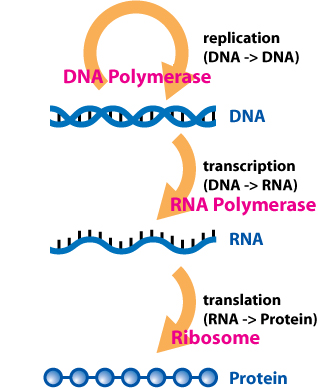
\includegraphics[width = 0.4\textwidth]{../images/Central_Dogma_of_Molecular_Biochemistry_with_Enzymes.jpg}
\caption{(Top) The genetic code, which dictates the conversion of RNA codons into amino acids. Codons are read from the inside of the figure outward. Three codons (\textnucl{UAA}, \textnucl{UAG}, and \textnucl{UGA}) do not have a corresponding amino acid and are called stop codons because when encountered they serve to halt translation. (Bottom) The central dogma of molecular biology states that molecular information flows from DNA in the nucleus, into the RNA that is transcribed from DNA, and then into proteins that are translated from RNA.}
\label{fig:central_dogma}
\end{figure}

%\begin{note}[%
%Like any dogma, there are times in which the central dogma of molecular biology is violated. If you are interested in an example, consider Chapter 4 of Bioinformatics Algorithms, https://www.bioinformaticsalgorithms.org/bioinformatics-chapter-4.
%]\end{note}

\phantomsection
\subsection{Transcription factors control gene regulation}

All of your cells have essentially the same DNA, and yet your liver cells, heart cells, and brain cells are able to serve different functions. This is because the rates at which these genes are \textdef{regulated}{gene regulation}{the process by which a gene can be activated or repressed (i.e., turned ``on'' or ``off'') via molecular mechanisms}, or converted into RNA and then protein, vary for different cell types and in response to different stimuli.

Gene regulation typically occurs at either the DNA or protein level. At the DNA level, regulation is modulated by \textdef{transcription factors}{transcription factor}{a protein serving to regulate genes by binding to DNA}, master regulator proteins that typically bind to the DNA immediately preceding a gene and serve to either \textdef{activate}{gene activation}{the process by which the production of a gene is increased} or \textdef{repress}{gene repression}{the process by which the production of a gene is decreased} the gene's rate of transcription, turning that rate up or down, respectively.

Because of the central dogma, transcription factors are involved in a feedback loop. DNA is transcribed into RNA, which is translated into the protein sequence of a transcription factor, which then binds to the region preceding a gene and changes its rate of transcription.

Transcription factors are vital for the cell's response to its environment because extracellular stimuli can serve to activate a transcription factor via a system of signaling molecules that convey a signal through relay molecules to the transcription factor (\autoref{fig:transduction}). Only when the transcription factor is activated will it regulate its target protein(s).\\

\begin{figure}[h]
\centering
\mySfFamily
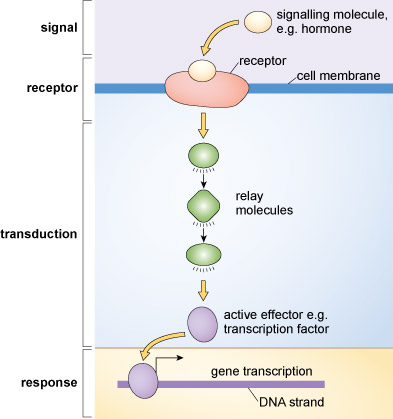
\includegraphics[width = 0.6\textwidth]{../images/signal_pathway.jpg}
\caption{A cell receiving a signal which triggers a response in which this signal is ``transduced'' into the cell, resulting in transcription of a gene.}
\label{fig:transduction}
\end{figure}

In \autoref{chapter:chemotaxis}, we will discuss the details of how the cell detects an extracellular signal and conveys it as a response within the cell. For now, we will focus on the relationship between transcription factors and the genes that they regulate.

\phantomsection
\subsection{Determining if a transcription factor regulates a given gene}

A transcription factor has a weak binding affinity to DNA in general, but it has a very strong binding affinity for a single specific short sequence of nucleotides called a \textdef{sequence motif}{sequence motif}{a repeated collection of nucleotides, which may serve as a binding site for a protein such as a transcription factor}. Think of a transcription factor as latching onto DNA and then ``sliding'' up and down the DNA molecule until it finds its target motif, where it clamps down. If this motif occurs immediately before a gene, then the transcription factor will regulate this gene.\\

\begin{note}[%
The astute reader will notice that we have already used the term ``motif'' in two different contexts, to mean both a recurring network substructure and (now) a sequence of nucleotides to which a transcription factor binds. This sequence is called a ``motif'' because the transcription factor may regulate multiple different genes, so that the binding sequence may occur immediately before all of these genes.
]\end{note}

A natural question, then, is to find the set of genes to which a transcription factor binds. A widespread experimental approach answering this question is called \textdef{ChIP-seq}{ChIP-seq}{short for ``chromatin immunoprecipitation sequencing'', an approach that }, which is short for \textdefnogloss{chromatin immunoprecipitation sequencing}. This approach, illustrated in \autoref{fig:ChIP-seq_workflow}, combines an organism's DNA with multiple copies of a protein of interest that binds to DNA (which in this case would be the transcription factor). After allowing for the proteins to bind naturally to the DNA, the DNA is cleaved into much smaller fragments of a few hundred base pairs. As a result, we obtain a collection of DNA fragments, some of which are attached to a copy of our protein of interest.

\begin{figure}[hp]
\centering
\mySfFamily
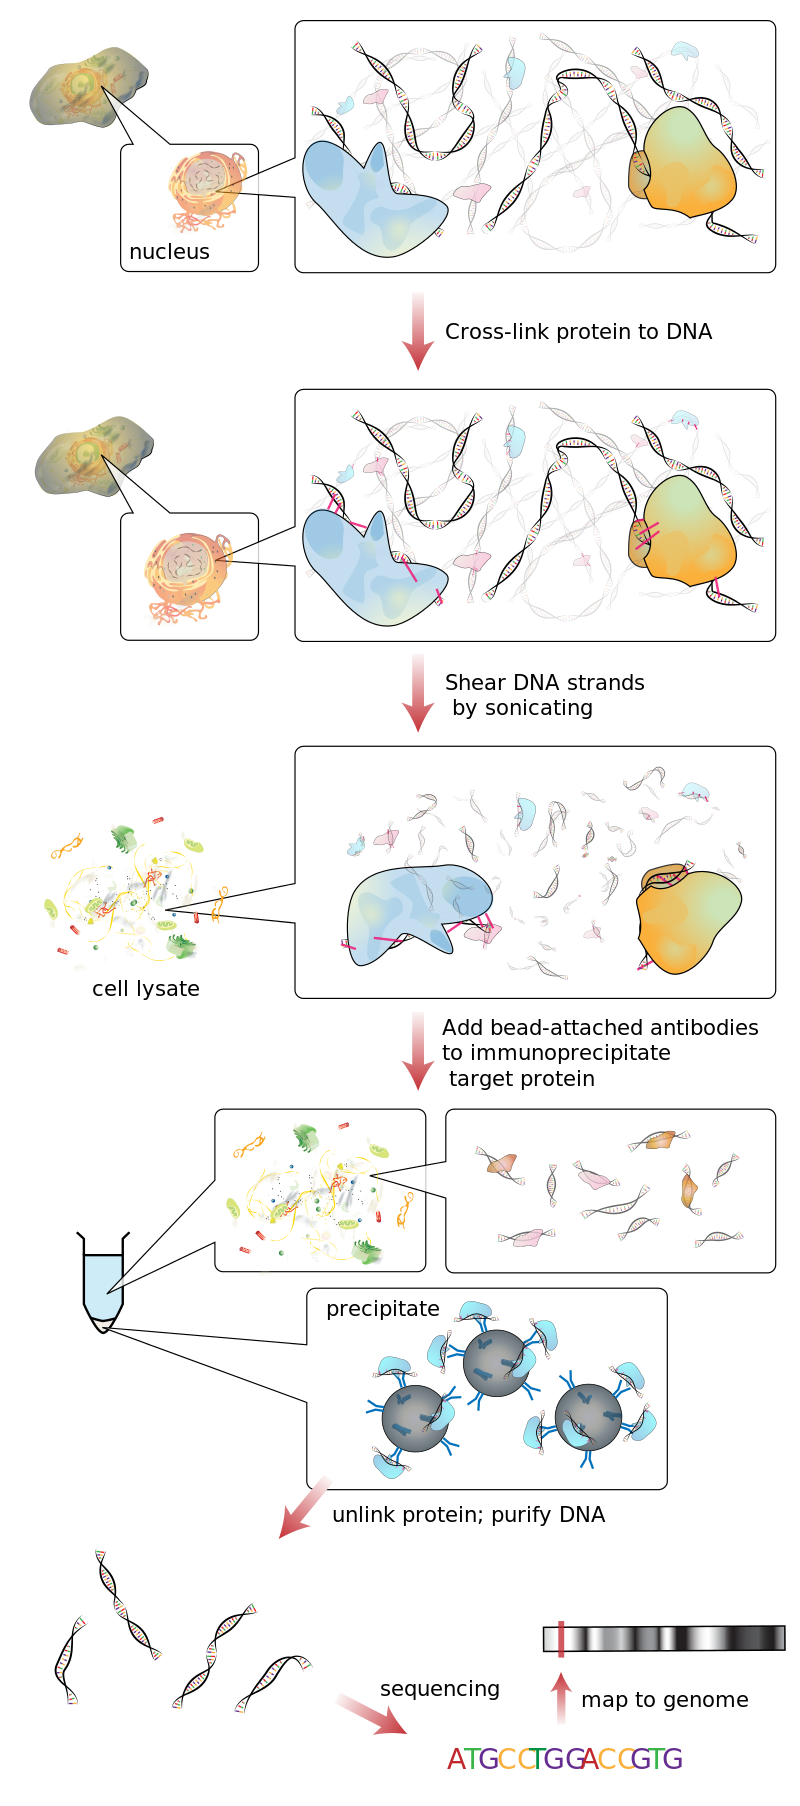
\includegraphics[width = 0.56\textwidth]{../images/ChIP-seq_workflow.png}
\caption{An overview of ChIP-seq.}
\label{fig:ChIP-seq_workflow}
\end{figure}

The question is how to isolate the fragments of DNA that are bound to a single transcription factor of interest, and the clever trick is to use an \textdef{antibody}{antibody}{a blood protein that binds to a specific foreign substance in the body}. Normally, antibodies are produced by the immune system to target foreign pathogens. The antibody used by ChIP-seq is designed to identify a single protein of interest, and the antibody is attached to a bead. Once the antibody attaches to the protein target, a single complex is formed consisting of the DNA fragment, the transcription factor bound to the DNA, the antibody that recognized the transcription factor, and the bead bound to the antibody. Because the bead weighs down these complexes, they can be filtered out as preciptate from the solution, and we are left with just the DNA fragments that are bound to our transcription factor.

In a final step, the protein is unlinked from the DNA, leaving a collection of DNA fragments that were previously bound to a single transcription factor. Each fragments is read using DNA sequencing to determine its order of nucleotides and then queried against the genome to determine the gene(s) that the fragment precedes. We can therefore postulate that these are the genes that the transcription factor regulates!\\

\begin{qbox}[%
How do you think that researchers could determine whether a transcription factor activates or represses a given gene?
]\end{qbox}

As a result of techniques like ChIP-seq, researchers have learned a great deal about which transcription factors regulate which genes. The key is to organize the relationships between transcription factors and the genes that they regulate in a way that will help us identify patterns in these relationships.\\


\FloatBarrier
\phantomsection

\section{Transcription Factor Networks}
\label{sec:transcription_factor_networks}
\phantomsection

\subsection{The transcription factor network of \textit{E. coli}}

Once we know which genes each transcription factor regulates, we can consolidate this information into a \textdef{transcription factor network}{transcription factor network}{a network whose nodes represent an organism's proteins, and such that a ``one-way'' directed edge connects one protein \textvar{X} to protein \textvar{Y} if \textvar{X} is a transcription factor that regulates \textvar{Y}}. The nodes in the network represent an organism's proteins, and we connect \textvar{X} to \textvar{Y} with an edge if \textvar{X} is a transcription factor that regulates the expression of protein \textvar{Y}. These edges are one-way connections; any node can have an edge leading into it, but only a transcription factor can have an edge leaving it.

\autoref{fig:e_coli_tf_network} shows a portion of the transcription factor network for \textit{Escherichia coli}, the workhorse model organism of bacterial study. The complete network, which is the sum of over two decades of biological research, consists of thousands of genes and around 300 transcription factors. Because of the size of this network, it forms what computational biologists affectionally call a ``hairball'', or a network with so many connections that it is functionally impossible to analyze visually. For this reason, we will need to use computational approaches to study this network.

Note that the edges in the \textit{E. coli} transcription factor network below are colored red or green. An edge connecting \textvar{X} to \textvar{Y} is colored green if \textvar{X} activates \textvar{Y}, and it is colored red if \textvar{X} represses \textvar{Y}. (Alternatively, we could label the edges with a ``+'' or ``$-$''.)\\

\begin{figure}[h]
\centering
\mySfFamily
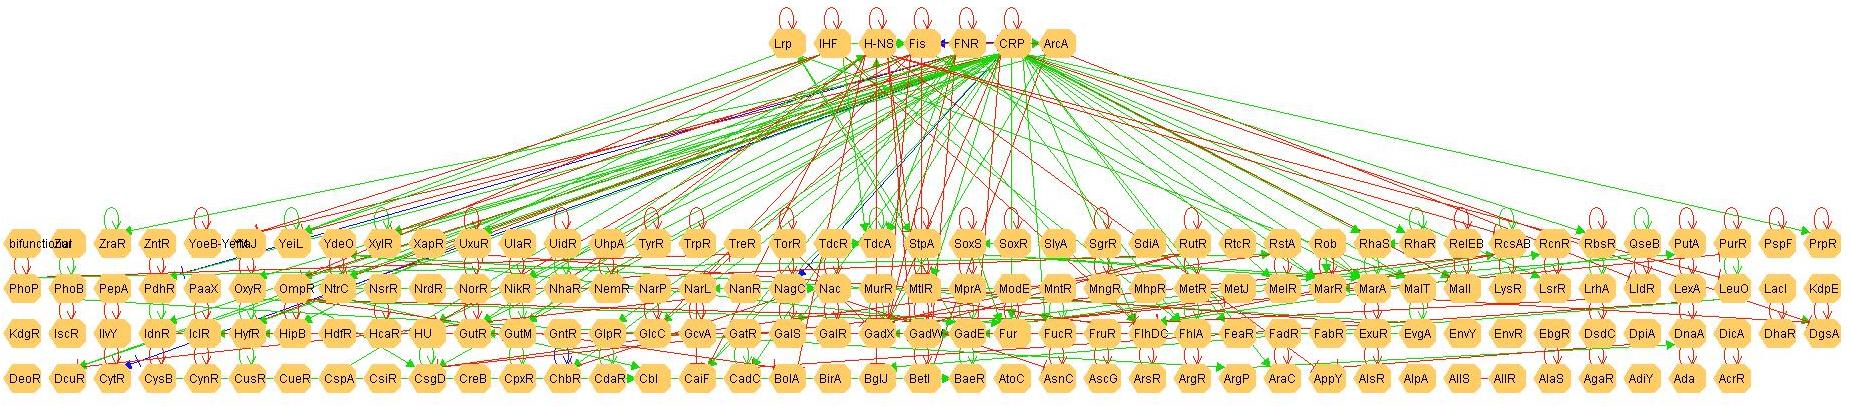
\includegraphics[width = 0.85\textwidth]{../images/e_coli_tf_network.jpeg}
\caption{A subset of the \textit{E. coli} transcription factor network. An edge from \textvar{X} to \textvar{Y} denotes that \textvar{X} is a transcription factor that regulates \textvar{Y}. Edges corresponding to activation are colored green, and edges corresponding to repression are colored red.}
\label{fig:e_coli_tf_network}
\end{figure}

\begin{qbox}[%
Do you notice anything interesting about the network in \autoref{fig:e_coli_tf_network}?
]\end{qbox}

\FloatBarrier
\phantomsection
\subsection{Loops in the transcription factor network}

You may have noticed that the \textit{E. coli} transcription factor network seems to have surprisingly many \textdef{loops}{loop}{an edge in a network connecting a node to itself}, or edges that connect a node to itself. We will pause to consider the implications of a loop in a transcription factor network --- what does it mean for a transcription factor to regulate itself?

A transcription factor is a protein, which means that because of the Central Dogma of Molecular Biology, the transcription factor is produced as the result of transcription and translation of a gene appearing in an organism's DNA. In \textdef{autoregulation}{autoregulation}{the process by which a transcription factor regulates its own production} (\autoref{fig:autoregulation_example}), the transcription factor protein then binds to the DNA in the region preceding the gene that encodes the very \textit{same} transcription factor. This type of \textit{feedback} is a beautiful and surprising feature of a simple biological system.

\begin{figure}[h]
\centering
\mySfFamily
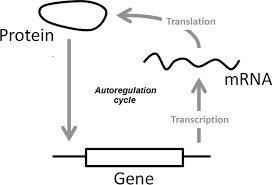
\includegraphics[width = 0.7\textwidth]{../images/autoregulation_example.png}
\caption{A simplified illustration of autoregulation, in which a gene is transcribed into messenger RNA (mRNA) and then translated into protein, and then this protein regulates the same gene, producing a feedback loop. ``Protein'' labels the transcription factor binding factor protein, which binds to the DNA encoding this transcription factor, labeled by ``Gene''.}
\label{fig:autoregulation_example}
\end{figure}

Transcription factor autoregulation leads us to ask two questions. First, how can we justify that a transcription factor network has ``surprisingly many'' loops? And second, if autoregulation is so common, then why would a transcription factor have evolved to regulate its own transcription? We will address these questions in each of the next two sections.\\


\FloatBarrier
\phantomsection

\section{Gene Autoregulation is Surprisingly Frequent}
\label{sec:gene_autoregulation_is_surprisingly_frequent}
\phantomsection

\subsection{Comparing a real transcription factor network against a random network}

To argue that a loop is indeed a motif in the \textit{E. coli} transcription factor network, we will apply a paradigm that occurs throughout computational biology (and science in general) when determining whether an observation is statistically significant. We will compare our observation against a  \textit{randomly generated} dataset; if the observation is frequent in a real dataset and rare in a random dataset, then it is likely to be statistically significant. Randomness saves the day again!\\

 \begin{qbox}[%
 How can we apply this paradigm of forming a randomly generated dataset to determine whether a transcription factor network contains a significant number of loops?
 ]\end{qbox}

To determine whether the number of loops in the transcription factor network of \textit{E. coli} is statistically significant, we will compare this number against the expected number of loops we would find in a randomly generated transcription factor network. If the former is much higher than the latter, then we have strong evidence that some selective force is causing gene autoregulation.

There are multiple ways to generate a random network, but we will use an approach developed by Edgar Gilbert in 1959. Given an integer \textvar{n} and a probability \textvar{p} (between 0 and 1), we form \textvar{n} nodes. Then, for every possible pair of nodes \textvar{X} and \textvar{Y}, we connect \textvar{X} to \textvar{Y} via a directed edge with probability \textvar{p}; that is, we simulate the process of flipping a weighted coin that has probability \textvar{p} of coming up ``heads''.\\

\begin{note}[%
Simulating a weighted coin flip amounts to generating a ``random'' number $x$ between 0 and 1, and considering it ``heads'' if $x$ is less than $p$ and ``tails'' otherwise. For more details on random number generation, consult Programming for Lovers (\url{http://programmingforlovers.com}).
]\end{note}

\begin{qbox}[%
What should \textvar{n} and \textvar{p} be if we are generating a random network to compare against the \textit{E. coli} transcription factor network?
]\end{qbox}

The full \textit{E. coli} transcription factor network contains thousands of genes, most of which are not transcription factors. As a result, the approach described above may form a random network that connects non-transcription factors to other nodes, which we should avoid.

Instead, we will focus on the network comprising only those \textit{E. coli} transcription factors that regulate each other. This network has 197 nodes and 477 edges, and so we will begin by forming a random network with $\textvar{n} = 197$ nodes.

We then select \textvar{p} to ensure that our random network will on average have 477 edges. To do so, we note that there are $\textvar{n}^2$ pairs of nodes that could have an edge connecting them (\textvar{n} choices for the starting node and \textvar{n} for the ending node). If we were to set \textvar{p} equal to $1/n^2$, then we would expect on average only to see a single edge in the random network. We therefore scale this value by 477 and set \textvar{p} equal to $477/n^2 \approx 0.0123$ so that we will see, on average, 477 edges in our random network.\tutorial[motifs/tutorial_loops]

\FloatBarrier
\phantomsection
\subsection{The negative autoregulation motif}

In a random network containing \textvar{n} nodes, the probability that a given edge is a loop is 1/\textvar{n}. Therefore, if the network has \textit{e} edges, then we would on average see \textit{e}/\textvar{n} loops in the network. In our case, \textvar{n} is 197, and \textit{e} is 477; therefore, on average, we expect to see $197/497 \approx 2.42$ loops in a random network. Yet the real \textit{E. coli} network of transcription factors that regulate each other contains 130 loops!

Furthermore, in a random network, we would expect about half of the edges correspond to activation, and the other half correspond to repression. But of the 130 loops in the \textit{E. coli} network, 35 correspond to activation and 95 correspond to repression. Just as you would be surprised to flip a coin 130 times and see ``heads'' come up 95 times, the cell must be \textdef{negatively autoregulating}{negative autoregulation}{the process in which a transcription factor represses itself} for some reason.

Why in the world would organisms have evolved the process of autoregulation only for a transcription factor to \textit{slow down} its own transcription? In the next section, we will begin to unravel the mystery.\\


\FloatBarrier
\phantomsection

\section{The Negative Autoregulation Motif}
\label{sec:the_negative_autoregulation_motif}
\phantomsection

\subsection{Simulating transcriptional regulation with a reaction-diffusion model}

Theodosius Dobzhansky famously wrote that ``nothing in biology makes sense except in the light of evolution.'' In the spirit of this quotation, there must be some evolutionary reason for the presence of the large number of negatively autoregulating \textit{E. coli} transcription factors that we identified in the previous section. Our goal is to use biological modeling to establish this justification.

We will simulate a ``race'' to the \textdef{steady state}{steady state}{also called equilibrium, a state in which potentially conflicting chemical forces are balanced}, or \textdefnogloss{equilibrium}, concentration of a transcription factor \textvar{Y} in two cells. In the first cell (\autoref{fig:two_cells} (left)), a transcription factor \textvar{X} activates \textvar{Y}; in the second cell (\autoref{fig:two_cells} (right)), \textvar{Y} also negatively autoregulates. Our premise is that the cell that reaches the steady state faster can respond more quickly to its environment and is therefore more fit for survival.\\

\begin{figure}[h]
\centering
\mySfFamily
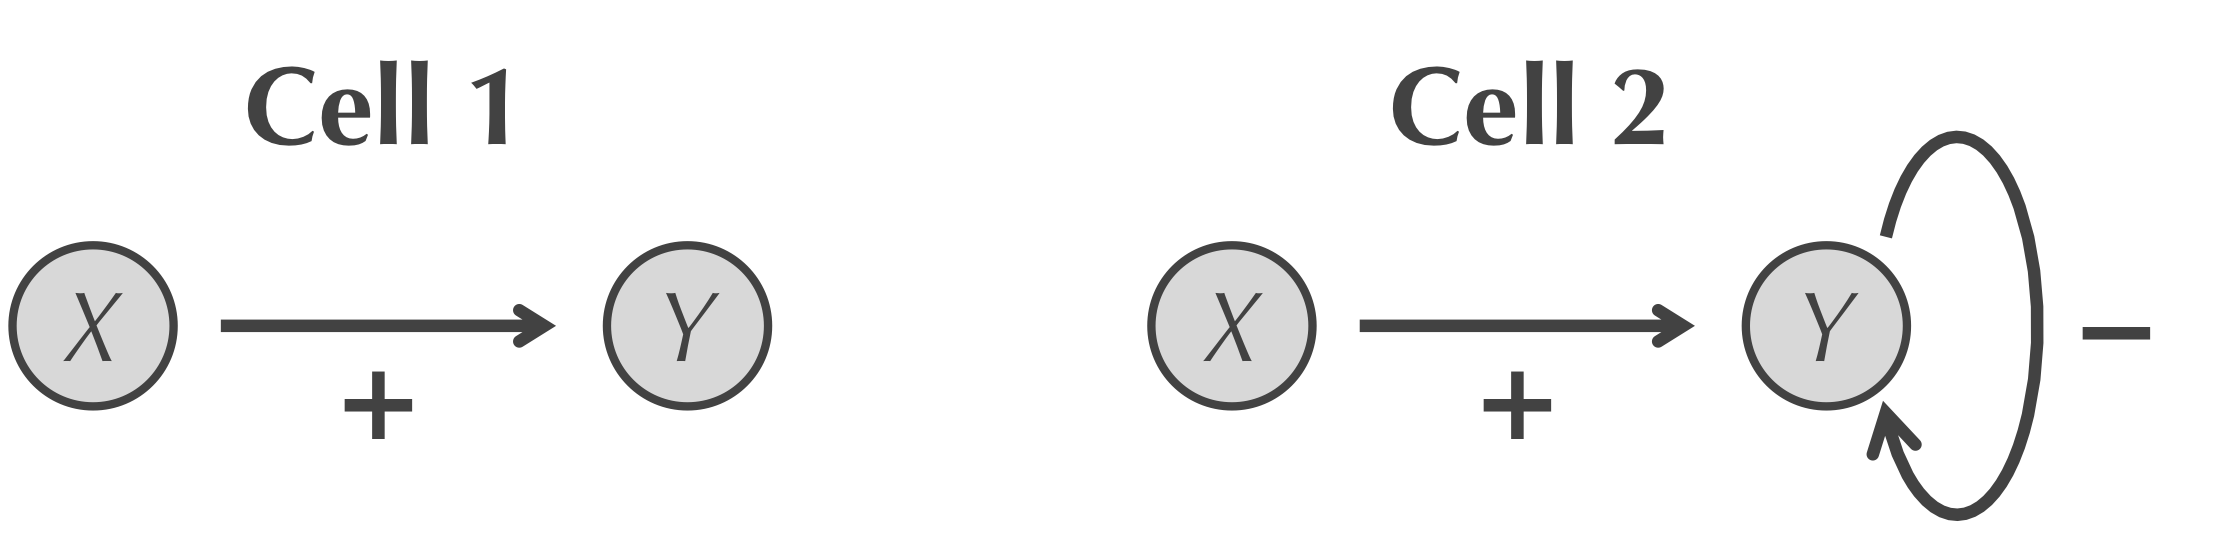
\includegraphics[width = 0.7\textwidth]{../images/two_cells.png}
\caption{The two cells that we wish to simulate. In the first cell (left), \textvar{X} only activates \textvar{Y}; in the second cell (right), \textvar{Y} also negatively autoregulates.}
\label{fig:two_cells}
\end{figure}

We will simulate these two cells using a reaction-diffusion model analogous to the one introduced in \autoref{chapter:turing}. For our new model, the ``particles'' represent the two transcription factors \textvar{X} and \textvar{Y}.

We begin with the first cell. To simulate \textvar{X} activating \textvar{Y}, we use the reaction $\textvar{X} \rightarrow \textvar{X} + \textvar{Y}$. In a given interval of time, there is a constant underlying probability related to the reaction rate that any given \textvar{X} particle will spontaneously form a new \textvar{Y} particle.

We should also account for the fact that proteins are \textit{degraded} over time by enzymes called proteases. The typical protein's concentration will be degraded by 20 to 40 percent in an hour, but transcription factors degrade even faster, lasting a matter of minutes. Degradation is an important feature  of cellular design, as it allows the cell to remove a protein after increasing that protein's concentration in response to some environmental change.

To model the degradation of \textvar{Y}, we add a ``kill'' reaction that removes \textvar{Y} particles at some rate. We will initialize our simulation with no \textvar{Y} particles and the \textvar{X} concentration at steady state; since \textvar{X} is being produced at a rate that exactly balances its degradation rate, we will not need to add reactions to the model simulating the production or degradation of \textvar{X}.

To complete the model of the first cell, diffusion of the \textvar{X} and \textvar{Y} particles is not technically necessary because no reaction in our model requires the collision of two or more particles. However, for the sake of biological correctness, we will allow both \textvar{X} and \textvar{Y} particles to diffuse through the system at the same rate.\\

\begin{qbox}[%
What chemical reaction could be used to simulate the negative autoregulation of \textvar{Y}?
]\end{qbox}

The model of the second cell will inherit all of the reactions from the first cell (with the same reaction rates) while adding negative autoregulation of \textvar{Y}. We will model negative autoregulation with the reaction $2\textvar{Y} \rightarrow \textvar{Y}$. That is, when two \textvar{Y} particles collide, there is some probability related to the reaction rate that one of the particles serves to remove the other, which mimics the process of a transcription factor turning off another copy of itself during negative autoregulation.

To recap, the simulations of both cells will include an initial concentration of \textvar{X} at steady state, diffusion of \textvar{X} and \textvar{Y}, removal of \textvar{Y}, and the reaction $\textvar{X} \rightarrow \textvar{X} + \textvar{Y}$. The second simulation, which includes negative autoregulation of \textvar{Y}, will add the reaction $2\textvar{Y} \rightarrow \textvar{Y}$. \tutorial[motifs/tutorial_nar]\\

\begin{note}[%
Although we are using a particle-based model to mimic regulation, it is not attempting to replicate specific chemical reactions. In reality, gene regulation is a complicated chemical process that involves a great deal of molecular machinery. The purpose of the model is to strip away what is not relevant and retain the essence of what is being modeled.
]\end{note}

\FloatBarrier
\phantomsection
\subsection{Ensuring a mathematically controlled comparison}

\autoref{fig:nar_unequal_chart} shows a plot over time of the concentration of \textvar{Y} particles in the two simulated cells, using red for the first cell and yellow for the second cell. By allowing \textvar{Y} to slow its own transcription, we wound up with a simulation in which the final concentration of \textvar{Y} was \textit{lower}. How could negative autoregulation possibly be useful?

\begin{figure}[h]
\centering
\mySfFamily
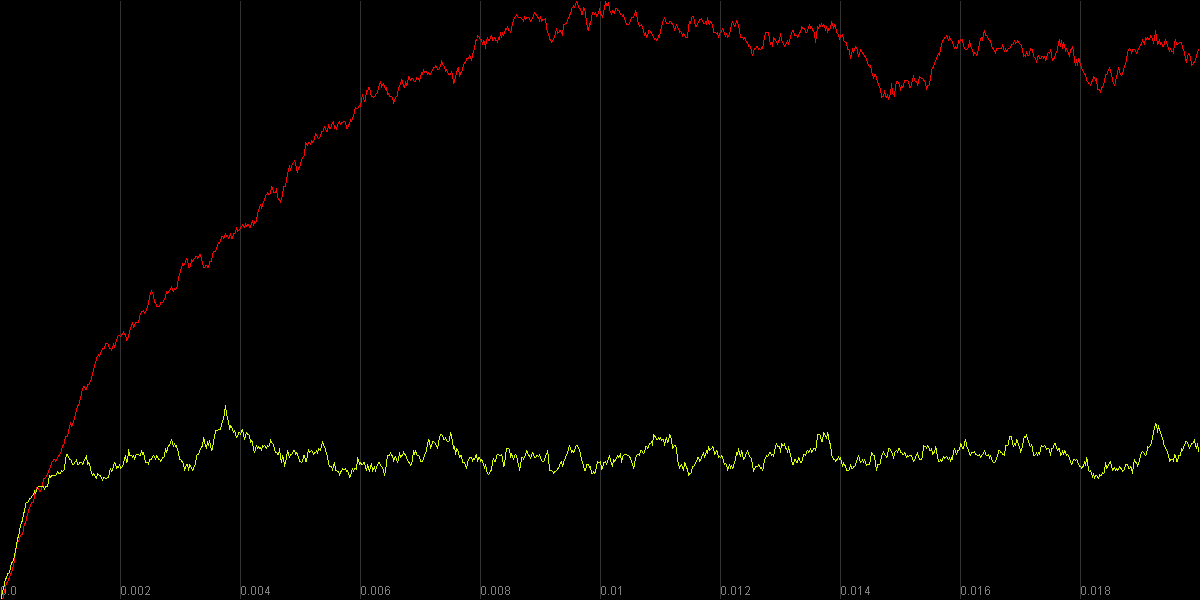
\includegraphics[width = 0.85\textwidth]{../images/cellblender_nar_unequal_chart.png}
\caption{A plot of the concentration of \textvar{Y} particles over time across two simulations. In the first cell (red), we only have activation of \textvar{Y} by \textvar{X}, whereas in the second cell (yellow), we keep all parameters fixed but add a reaction simulating the negative autoregulation of \textvar{Y}.}
\label{fig:nar_unequal_chart}
\end{figure}

The solution to this quandary is that the model we built was not a fair comparison between the two systems. In particular, the two simulations should converge to approximately the \textit{same} steady state concentration of \textvar{Y}, since achieving this concentration represents the cell's response to some stimulus. Ensuring this equal footing for the two simulations is called a \textdef{mathematically controlled comparison}{mathematically controlled comparison}{two models in which as many variables as possible are preserved between the two systems in an effort to preserve a fair comparison}.\\

\begin{qbox}[%
How can we change the parameters of our models to obtain a mathematically controlled comparison of the two simulated cells?
]\end{qbox}

We should keep a number of parameters constant across the two simulations because they are unrelated to regulation: the diffusion rates of \textvar{X} and \textvar{Y}, the number of initial particles \textvar{X} and \textvar{Y}, and the degradation rate of \textvar{Y}. With these parameters fixed, the only way that the final steady state concentration of \textvar{Y} can be the same in the two simulations is if we \textit{increase} the rate at which the reaction $\textvar{X} \rightarrow \textvar{X} + \textvar{Y}$ takes place in the simulation of the second cell.\tutorial[motifs/tutorial_nar_mathematically_controlled]

\autoref{fig:nar_equal_chart} plots the concentration of \textvar{Y} particles for the two simulated cells after ensuring a mathematically controlled comparison, in which the rate of the $\textvar{X} \rightarrow \textvar{X} + \textvar{Y}$ reaction has been increased in the second cell. This figure shows that the two simulated cells now have approximately the same steady state concentration of \textvar{Y}. However, the second cell reaches this concentration faster; that is, its \textdef{response time}{response time}{the time required for a biological system to respond to a stimulus (e.g., reaching a steady state concentration of a specific particle)} to the external stimulus causing an increase in the production of \textvar{Y} is shorter.

\begin{figure}[h]
\centering
\mySfFamily
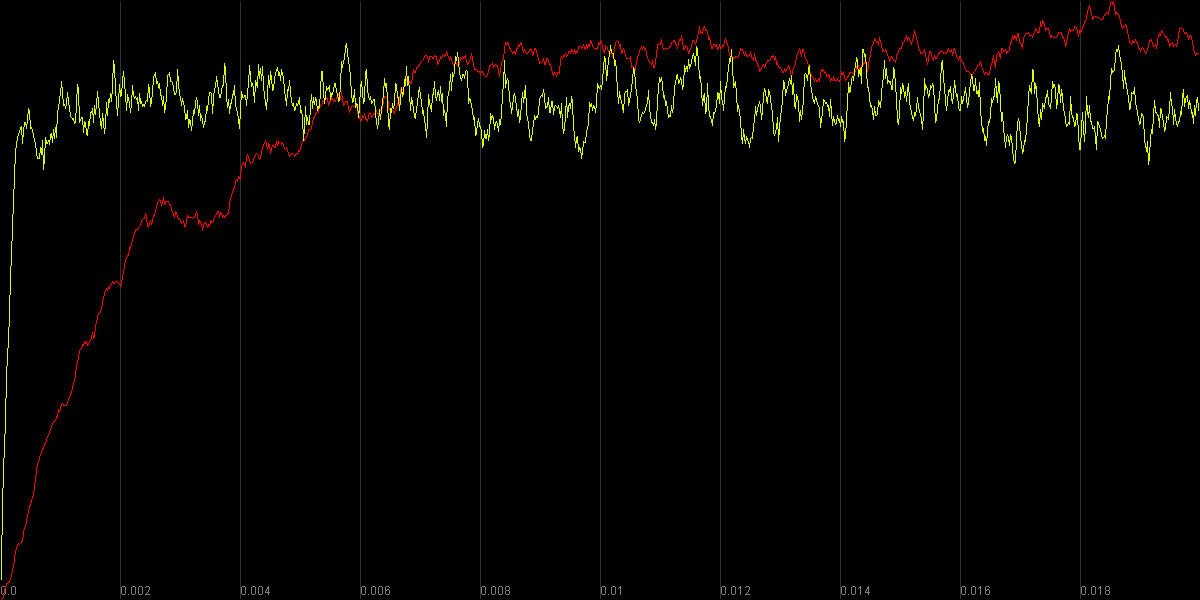
\includegraphics[width = 0.85\textwidth]{../images/cellblender_nar_equal_chart.png}
\caption{A plot of the concentration of \textvar{Y} particles across the same two simulations from \autoref{fig:nar_unequal_chart}. This time, in the second simulation (yellow), we increase the rate of the reaction $\textvar{X} \rightarrow \textvar{X} + \textvar{Y}$.  As a result, the two simulations have approximately the same steady state concentration of \textvar{Y}, and the simulation that includes negative autoregulation reaches steady state more quickly.}
\label{fig:nar_equal_chart}
\end{figure}

The plots in \autoref{fig:nar_equal_chart} also provide evidence of \textit{why} negative autoregulation may have evolved. The simulated cell including negative autoregulation wins the ``race'' to a steady state concentration of \textvar{Y}, and so we can conclude that a cell in which this transcription factor is negatively autoregulated is more fit for survival than one that does not. Uri Alon has proposed an excellent analogy of a negatively autoregulating transcription factor as a sports car that has both a powerful engine (corresponding to the higher rate of the reaction producing \textvar{Y}) and sensitive brakes (corresponding to negative autoregulation slowing the production of \textvar{Y} to reach equilibrium quickly).\\

\FloatBarrier
\phantomsection

\section{The Feedforward Loop Motif}
\label{sec:the_feedforward_loop_motif}
\phantomsection

\subsection{Feedforward loops}

In the previous section, we saw that negative autoregulation can be used to lower the response time of a protein to an external stimulus. But the cell can only use autoregulation to respond quickly if the autoregulated protein is itself a transcription factor. Only about 300 out of 4,400 total \textit{E. coli} proteins are transcription factors. How can the cell speed up the manufacture of a protein if that protein is not a transcription factor?

The answer lies in another transcription factor network motif called the \textdef{feedforward loop (FFL)}{feedforward loop (FFL)}{a network substructure in which \textvar{X} is connected to both \textvar{Y} and \textvar{Z}, and \textvar{Y} is connected to \textvar{Z}}. Shown in \autoref{fig:feed-forward_loop}, an FFL is a network substructure in which \textvar{X} is connected to both \textvar{Y} and \textvar{Z}, and \textvar{Y} is connected to \textvar{Z}. Calling the FFL motif a ``loop'' is a misnomer. Rather, it is a small structure in which there are two paths from \textvar{X} to \textvar{Z}; one via direct regulation of \textvar{Z} by \textvar{X}, and another with an intermediate transcription factor \textvar{Y}.

\begin{figure}[h]
\centering
\mySfFamily
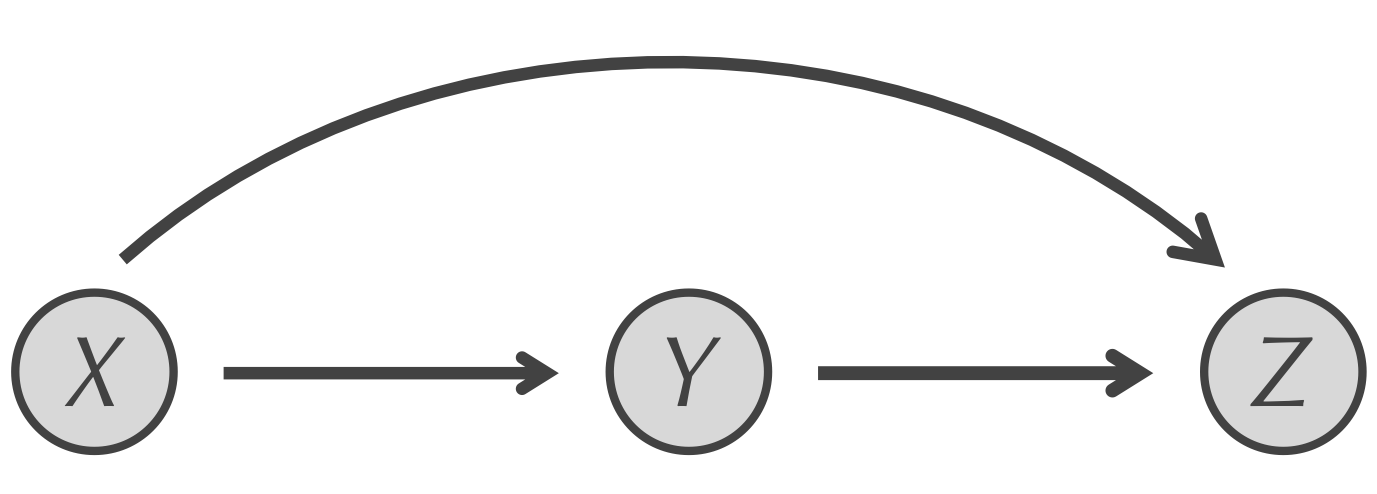
\includegraphics[width = 0.5\textwidth]{../images/feed-forward_loop.png}
\caption{The feedforward loop (FFL) motif. \textvar{X} regulates both \textvar{Y} and \textvar{Z}, and \textvar{Y} regulates \textvar{Z}.}
\label{fig:feed-forward_loop}
\end{figure}

Note that \textvar{X} and \textvar{Y} must be transcription factors because they have edges leading out from them, but \textvar{Z} does not have to be a transcription factor (and in fact typically is not). There are 42 FFLs in the transcription factor network of \textit{E. coli}; we leave the verification that this number is significant as an exercise.

Among the 42 total FFLs in the \textit{E. coli} transcription factor network, five of them have the structure in \autoref{fig:type-1_incoherent_feed-forward_loop}, in which the edges connecting \textvar{X} to \textvar{Y} and \textvar{X} to \textvar{Z} are assigned a ``+'' (activation) and the edge connecting \textvar{Y} to \textvar{Z} is assigned a ``$-$'' (repression). This specific form of the FFL motif is  called a \textdefnogloss{type-1 incoherent feedforward loop} and will be our focus for the rest of the section.\\

\begin{qbox}[%
How could we simulate a type-1 incoherent feedforward loop with a particle-based reaction-diffusion model akin to the simulation that we used for negative autoregulation? What would we compare this simulation against?
]\end{qbox}

\begin{figure}[h]
\centering
\mySfFamily
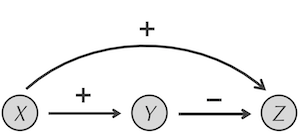
\includegraphics[width = 0.5\textwidth]{../images/type-1_incoherent_feed-forward_loop.png}
\caption{The incoherent feed-forward loop network motif. \textvar{X} activates \textvar{Y} and \textvar{Z}, while \textvar{Y} represses \textvar{Z}.}
\label{fig:type-1_incoherent_feed-forward_loop}
\end{figure}

\FloatBarrier
\phantomsection
\subsection{Modeling a type-1 incoherent feedforward loop}

As we did for negative autoregulation, we will simulate two cells and examine the concentration of a particle of interest, which in this case will be \textvar{Z}. The first cell will have a simple activation of \textvar{Z} by \textvar{X}, meaning that we will assume \textvar{X} starts at its steady state concentration and that \textvar{Z} is produced by the reaction $\textvar{X} \rightarrow \textvar{X} + \textvar{Z}$ and removed by a degradation reaction.

The second cell will include both of these reactions in addition to the reaction $\textvar{X} \rightarrow \textvar{X} + \textvar{Y}$ to model the activation of \textvar{Y} by \textvar{X}, along with the new reaction $\textvar{Y} + \textvar{Z} \rightarrow \textvar{Y}$ to model the repression of \textvar{Z} by \textvar{Y}. Because \textvar{Y} and \textvar{Z} are being produced from a reaction, we will also have degradation reactions for \textvar{Y} and \textvar{Z}. For the sake of fairness, we will use the same kill rates for both \textvar{Y} and \textvar{Z}.

Furthermore, to obtain a mathematically controlled comparison, the reaction $\textvar{X} \rightarrow \textvar{X} + \textvar{Z}$ should have a higher rate in the second simulation modeling the FFL. If we do not raise the rate of this reaction, then the repression of \textvar{Z} by \textvar{Y} will cause the steady state concentration of \textvar{Z} to be lower in the second simulation.\tutorial[motifs/tutorial_feed]

\autoref{fig:ffl_chart} shows a plot visualizing the concentration of \textvar{Z} across the two simulations. As with negative autoregulation, the type-1 incoherent FFL allows the cell to ramp up production of a gene \textvar{Z} much faster than it would under simple regulation.\\

\begin{figure}[h]
\centering
\mySfFamily
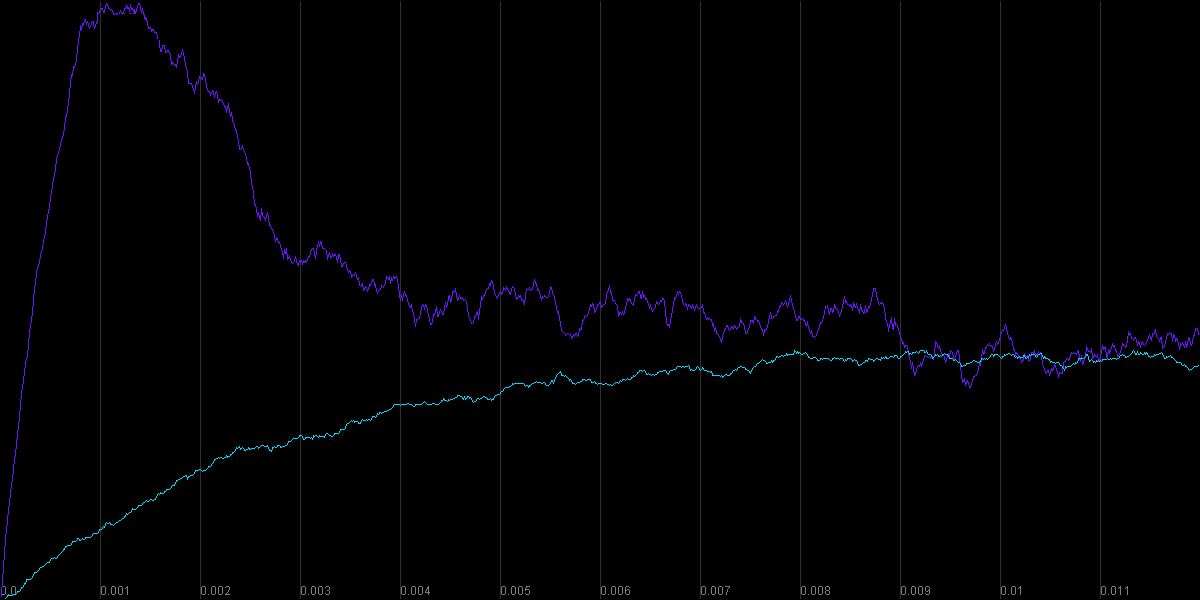
\includegraphics[width = 0.85\textwidth]{../images/cellblender_ffl.png}
\caption{The concentration of \textvar{Z} in the two simulations. Simple activation of \textvar{Z} by \textvar{X} is shown in blue, and the type-1 incoherent FFL is shown in purple.}
\label{fig:ffl_chart}
\end{figure}

However, you will note a slightly different pattern to the growth of \textvar{Z} than we saw under negative autoregulation. When modeling negative autoregulation, the concentration of the protein approached steady state from below. In the case of the FFL, the concentration of \textvar{Z} grows so quickly that it passes its eventual steady state concentration and then returns to this steady state from above.

We can interpret from the model why the FFL allows for a fast response time as well as why it initially passes the steady state concentration. At the start of the simulation, \textvar{Z} is activated by \textvar{X} very quickly. \textvar{X} regulates the production of \textvar{Y} as well, but at a lower rate than the regulation of \textvar{Z} because \textvar{Y} only has its own degradation to slow this process. Therefore, more \textvar{Z} is initially produced than \textvar{Y}, which causes the concentration of \textvar{Z} to shoot past its eventual steady state.

\autoref{fig:ffl_chart} is reminiscent of a \textdefnogloss{damped oscillation} process like the one in \autoref{fig:damped_oscillator}, in which the concentration of a particle oscillates above and below a steady state, while the amplitude of the wave gets smaller and smaller. Is it possible for a network motif to produce more of a true ``wave'' without dampening?\\

\begin{figure}[h]
\centering
\mySfFamily
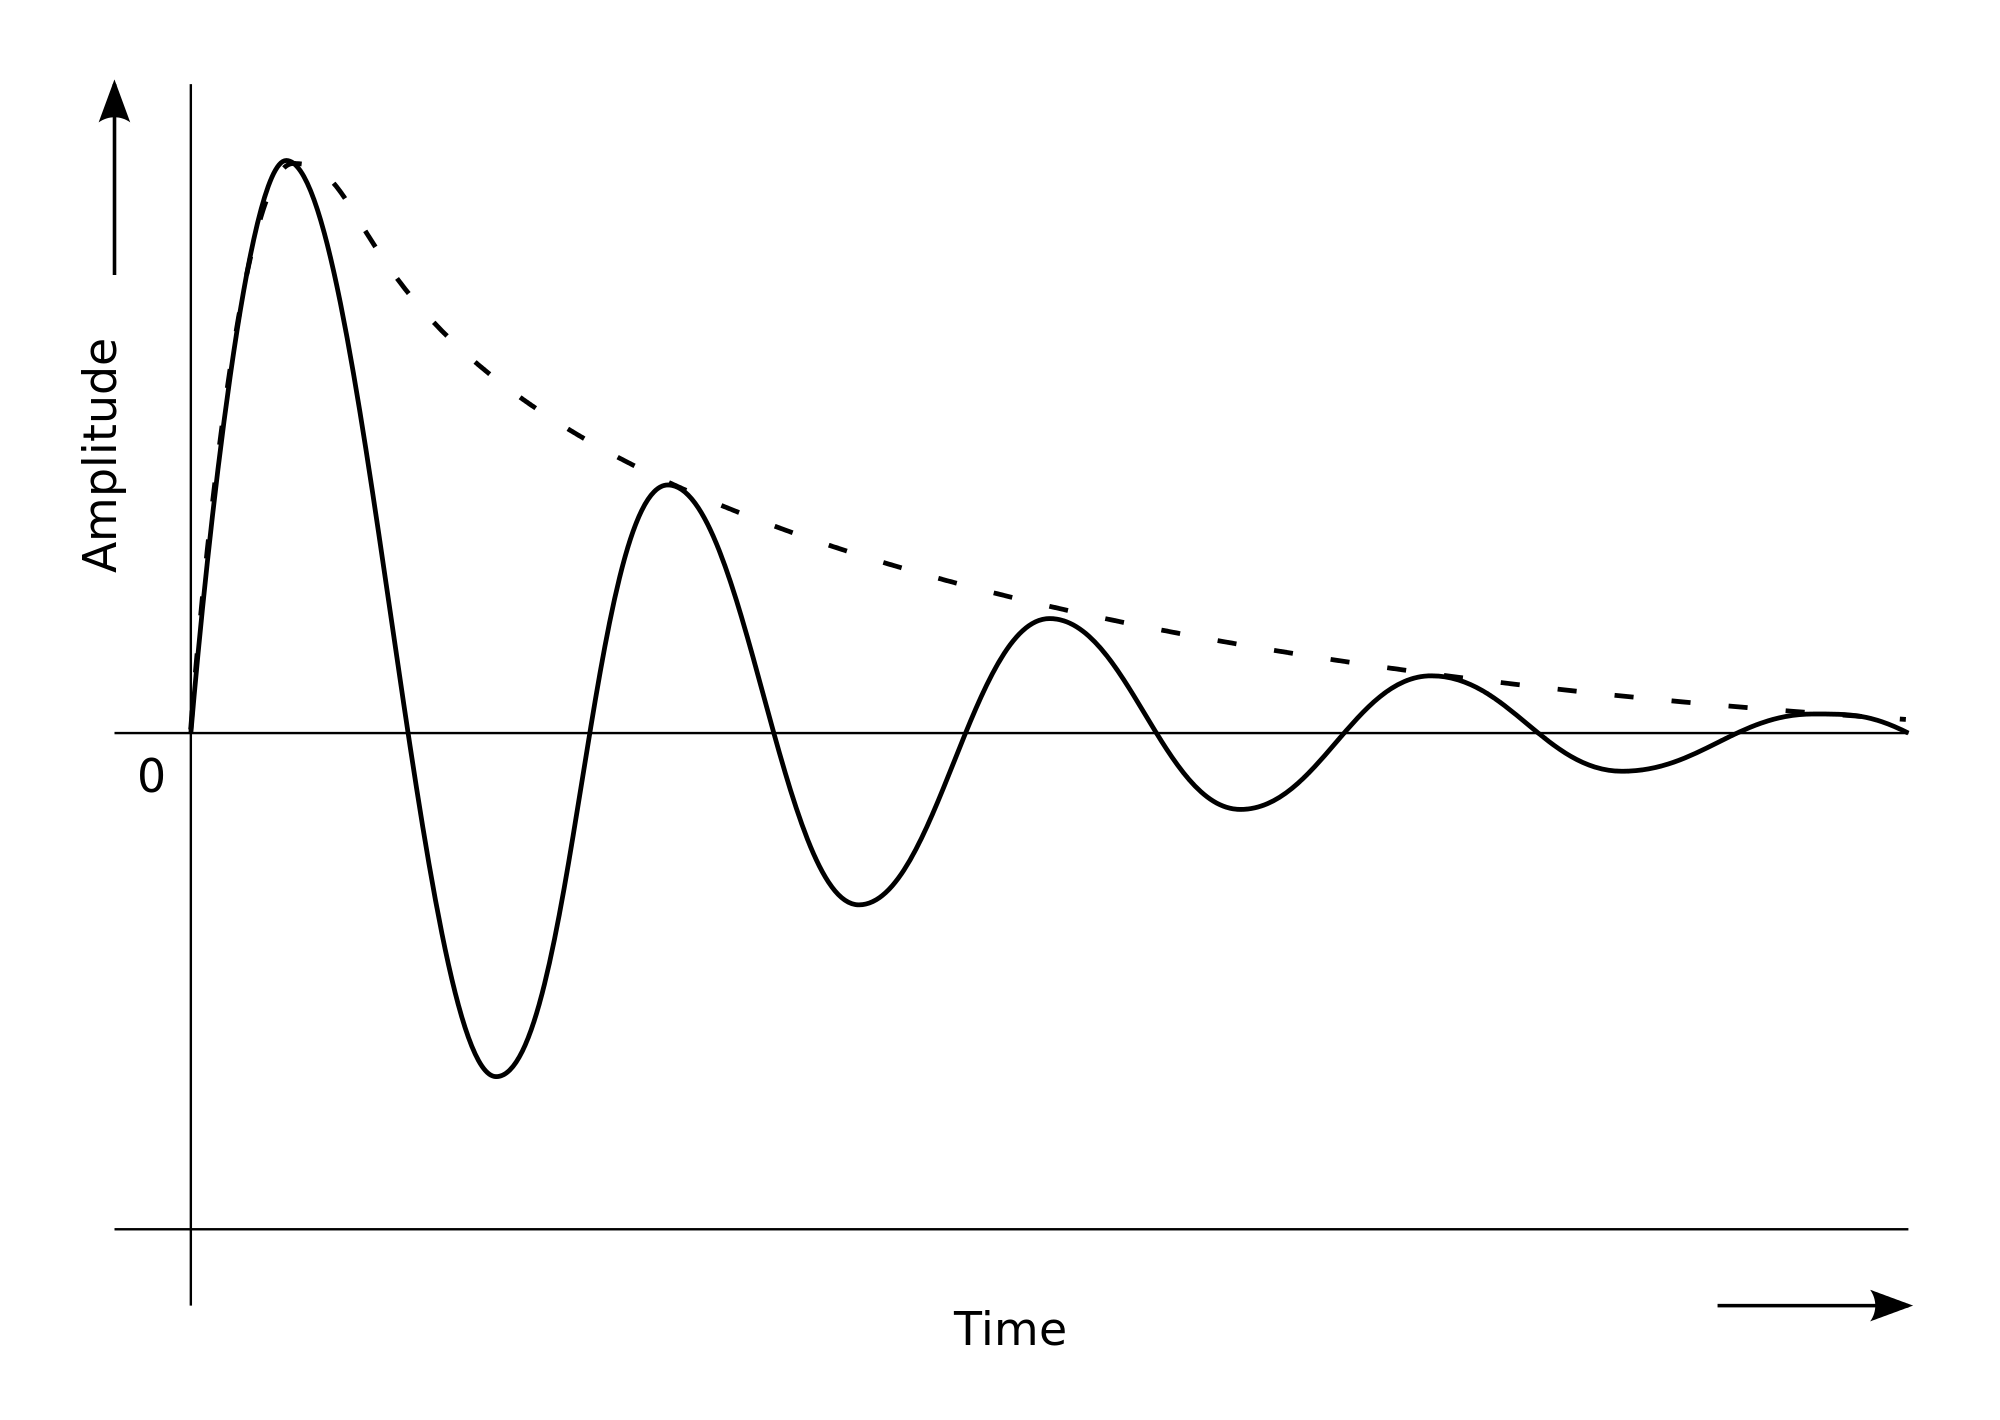
\includegraphics[width = 0.7\textwidth]{../images/damped_oscillator.png}
\caption{In a damped oscillation, the value of some variable (shown on the y-axis) oscillates back and forth around an asymptotic value while the amplitude decreases over time.}
\label{fig:damped_oscillator}
\end{figure}

\FloatBarrier
\phantomsection

\section{Biological Oscillators}
\label{sec:biological_oscillators}
\phantomsection

\subsection{Oscillators are everywhere in nature}

Even if placed in a windowless bunker without clocks, humans will maintain a roughly 24-hour cycle of sleep and wakefulness. This \textdef{circadian rhythm}{circadian rhythm}{a collection of internal changes in living things that follow a roughly 24-hour cycle} is present throughout many living things, including plants and even cyanobacteria. Your heart and respiratory system also follow subconscious cyclical rhythms, and your cells are governed by a strict cell cycle as they grow and divide.

We might guess from what we have learned in this section that cyclical biological rhythms must be governed by simple rules. However, the question remains as to what these rules are and how they can correctly execute oscillations over and over.

Researchers have identified many network motifs that facilitate oscillation, some of which are very complicated and include many components. In this section, we will focus on a simple three-component oscillator motif.

\FloatBarrier
\phantomsection
\subsection{The repressilator: a synthetic biological oscillator}

The \textdef{repressilator}{repressilator motif}{a transcription factor network motif in which \textvar{X} represses \textvar{Y}, \textvar{Y} represses \textvar{Z}, and \textvar{Z} represses \textvar{X}} is shown in \autoref{fig:repressilator}. In this motif, all three proteins are transcription factors, and they form a cycle in which \textvar{X} represses \textvar{Y}, \textvar{Y} represses \textvar{Z}, and \textvar{Z} represses \textvar{X}. The repressilator forms a feedback loop, but nothing \textit{a priori} about this motif would indicate that it would lead to oscillation.\\

\begin{figure}[h]
\centering
\mySfFamily
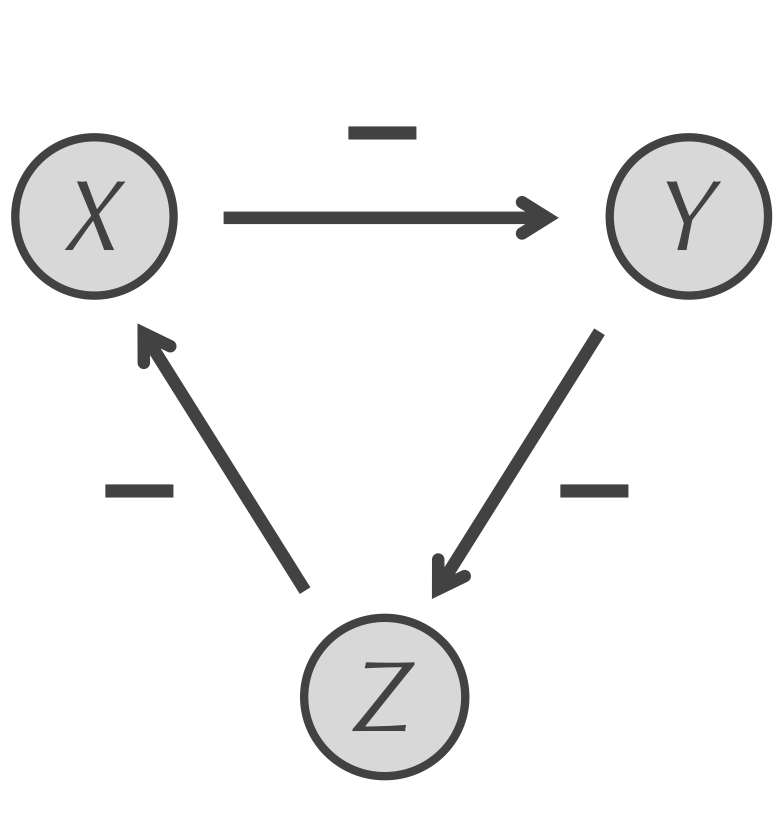
\includegraphics[width = 0.3\textwidth]{../images/repressilator.png}
\caption{The repressilator motif for three particles \textvar{X}, \textvar{Y}, and \textvar{Z}. \textvar{X} represses \textvar{Y}, which represses \textvar{Z}, which in turn represses \textvar{X}, forming a feedback loop.}
\label{fig:repressilator}
\end{figure}

\begin{qbox}[%
Devise a reaction-diffusion model representing the repressilator.
]\end{qbox}

To build a reaction-diffusion model accompanying the repressilator, we start with a quantity of \textvar{X} particles and no \textvar{Y} or \textvar{Z} particles. We assume that all three particles diffuse at the same rate and degrade at the same rate.

Furthermore, we assume that all three particles are produced as the result of an activation process by some other transcription factor(s), which we assume happens at the same rate. We will use a single \textdefnogloss{hidden particle} \textvar{I} that serves to activate the three visible particles via the three reactions $\textvar{I} \rightarrow \textvar{I} + \textvar{X}$, $\textvar{I} \rightarrow \textvar{I} + \textvar{Y}$, and $\textvar{I} \rightarrow \textvar{I} + \textvar{Z}$, all taking place at the same rate.

When discussing the feed-forward loop, we saw that we can use the reaction $\textvar{X} + \textvar{Y} \rightarrow \textvar{X}$ to model the repression of \textvar{Y} by \textvar{X}. To complete the repressilator model, we will supplement this reaction with the two reactions $\textvar{Y} + \textvar{Z} \rightarrow \textvar{Y}$ and $\textvar{Z} + \textvar{X} \rightarrow \textvar{Z}$, with all three repression reactions occurring at the same rate.\tutorial[motifs/tutorial_oscillators]

\FloatBarrier
\phantomsection
\subsection{Interpreting the repressilator's oscillations}

\autoref{fig:repressilator_chart} plots the concentration over time of \textvar{X}, \textvar{Y}, and \textvar{Z} particles from our repressilator simulation (colored yellow, red, and blue, respectively). The system exhibits clear oscillatory behavior, with \textvar{X}, \textvar{Y}, and \textvar{Z} taking turns being at high concentration.\\

\begin{qbox}[%
Why do you think that the repressilator motif leads to this pattern of oscillations?
]\end{qbox}

\begin{figure}[h]
\centering
\mySfFamily
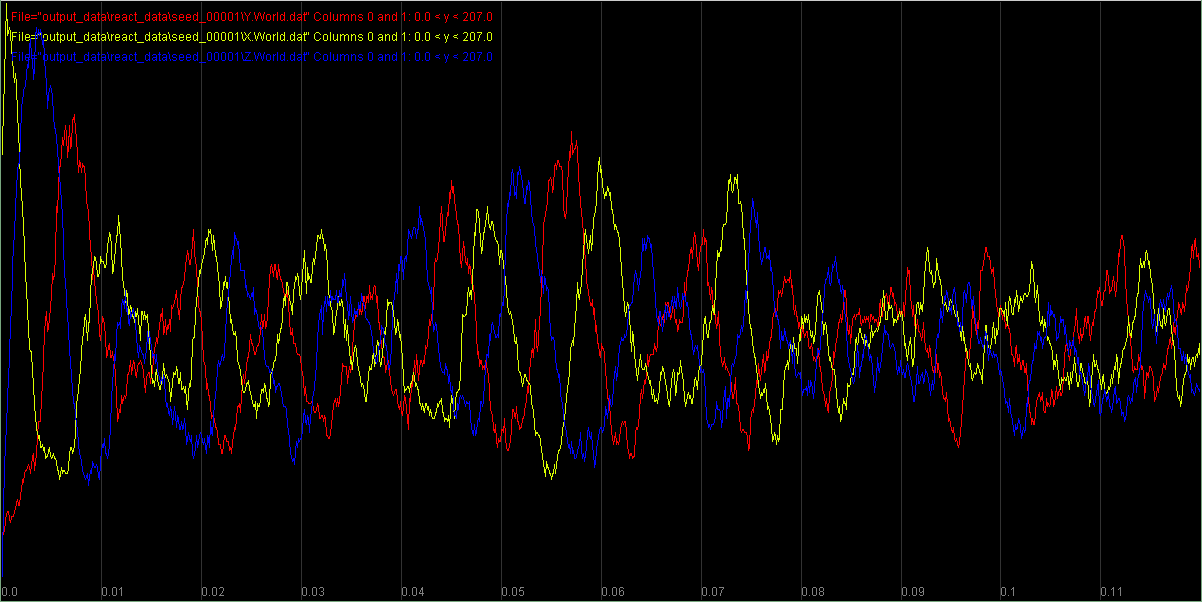
\includegraphics[width = 0.85\textwidth]{../images/repressilator_chart.png}
\caption{Modeling the repressilator's concentration of particles over time; \textvar{X} is shown in yellow, \textvar{Y} is shown in red, and \textvar{Z} is shown in blue}
\label{fig:repressilator_chart}
\end{figure}

Because the concentration of \textvar{X} starts out high, with no \textvar{Y} or \textvar{Z} present, the concentration of \textvar{X} briefly increases because its rate of production exceeds its rate of degradation. With no \textvar{Y} or \textvar{Z} particles present, there are none to degrade or be repressed, and so the concentrations of these particles start increasing as well. However, because \textvar{X} particles begin at high concentration, the repression reaction $\textvar{X} + \textvar{Y} \rightarrow \textvar{X}$ prevents the concentration of \textvar{Y} from growing as fast as the concentration of \textvar{Z}.

As the concentration of \textvar{Z} rises, the repression reaction $\textvar{Z} + \textvar{X} \rightarrow \textvar{Z}$ occurs often enough for the rate of removal of \textvar{X} to equal and exceed its rate of production, accounting for the first peak in \autoref{fig:repressilator_chart}. The concentration of \textvar{X} then plummets, with the concentration of \textvar{Z} rising up to replace it. This situation is shown by the second (blue) peak in \autoref{fig:repressilator_chart}.

As a result, \textvar{Z} and \textvar{X} have switched roles. Because there is a high concentration of \textvar{Z}, and the concentration of \textvar{Y} is increasing, the reaction $\textvar{Y} + \textvar{Z} \rightarrow \textvar{Y}$ will be frequent and reduce the concentration of \textvar{Z}. Furthermore, because the concentration of \textvar{X} has decreased, and the concentration of \textvar{Y} is still relatively low, the reaction $\textvar{X} + \textvar{Y} \rightarrow \textvar{X}$ will occur less often, allowing the concentration of \textvar{Y} to continue to rise. Eventually, the decrease in the concentration of \textvar{Z} and the increase in the concentration of \textvar{Y} will account for the third (red) peak in \autoref{fig:repressilator_chart}.

At this point, the reaction $\textvar{X} + \textvar{Y} \rightarrow \textvar{X}$ will suppress the concentration of \textvar{Y}. Because the concentrations of \textvar{X} and \textvar{Z} are both lower than the concentration of \textvar{Z}, the reaction $\textvar{Z} + \textvar{X} \rightarrow \textvar{Z}$ will not greatly influence the concentration of \textvar{X}, which will rise to meet the following concentration of \textvar{Y}, and we have returned to our original situation, at which point the cycle will begin again.

\FloatBarrier
\phantomsection
\subsection{Noise is a feature, not a bug}

Take another look at the oscillations of the repressilator in \autoref{fig:repressilator_chart}. You will notice that the concentrations zigzag as they travel up or down, and that they peak at slightly different levels each time.

This noise in the repressilator's oscillations is due to random variation as the particles bounce around due to diffusion. The repression reactions require two particles to collide in order for the reaction to take place. Due to random chance, these collisions may occur more or less often than expected because of random chance. Much of this noise is due to low sample size: we have around 150 molecules at each peak in the \autoref{fig:repressilator_chart}, but a given cell may have on the order of 1,000 to 10,000 molecules of a single protein.

The noise in the repressilator's oscillations is a feature, not a bug. As we have discussed previously, the cell's molecular interactions are inherently random. If we see oscillations in a simulation built on randomness, then we can be confident that this simulation is \textit{robust} to a certain amount of variation. We will further explore this robustness in the chapter's conclusion.\\

\FloatBarrier
\phantomsection

\section{Conclusion: The Robustness of Biological Oscillators}
\label{sec:biological_oscillators_must_be_robust}
\phantomsection

\subsection{Biological oscillators must be robust}

If your heart skips a beat when you are watching a horror movie, then it should return quickly to its natural rhythm. When you hold your breath to dive underwater, your normal breathing resumes at the surface. And regardless of what functions your cells perform or what disturbances they find in their environment, they should be able to maintain a normal cell cycle.

An excellent illustration of oscillator robustness is the body's ability to handle jet lag. There is no apparent reason why humans would have evolved to be able to fly halfway around the world. And yet our circadian clock is so resilient that after a few days of fatigue and crankiness, our circadian clock returns to a normal daily cycle.

In the previous section, we saw that the repressilator, a three-element motif, can exhibit oscillations even in a noisy environment of randomly moving particles. The repressilator's resilience makes us wonder how well it can respond to a disturbance in the concentrations of its particles.

\FloatBarrier
\phantomsection
\subsection{A coarse-grained repressilator model}

With our work on Turing patterns in \autoref{chapter:turing}, we saw that tracking the movements of many individual particles led to a slow simulation that did not scale well given more particles or reactions. This observation led us to devise a coarse-grained reaction-diffusion model that was still able to produce Turing patterns. We used a cellular automaton because the concentrations of particles varied in different locations and were diffusing at different rates.

We would like to devise a coarse-grained model of the repressilator. However, the particles diffuse at the same rate and are \textit{uniform} across the simulation, and so there is no need to track concentrations in individual locations. As a result, we will use a simulation that assumes that the particles are \textdefnogloss{well-mixed}.

For example, say that we are modeling a degradation reaction. If we start with a concentration of 10,000 \textvar{X} particles, then after a single time step, we will simply multiply the number of \textvar{X} particles by $(1-k)$, where \textit{k} is a parameter related to the rate of the degradation reaction.

As for a repression reaction like $\textvar{X} + \textvar{Y} \rightarrow \textvar{X}$, we can update the concentration of \textvar{Y} particles by subtracting some factor \textit{r} times the current concentrations of \textvar{X} and \textvar{Y} particles.

We will further discuss the technical details behind a well-mixed reaction-diffusion model in \autoref{chapter:chemotaxis}. In the meantime, we would like to see what happens when we make a major disturbance to the concentration of one of the particles in the well-mixed model. Do the particle concentrations resume their oscillations?\tutorial[motifs/tutorial_perturb]

\FloatBarrier
\phantomsection
\subsection{The repressilator is robust to disturbance}

\autoref{fig:nf_sim_interrupted_chart} shows plots over time of concentrations of each particle in our well-mixed simulation of the repressilator.  Midway through this simulation, we greatly increase the concentration of \textvar{Y} particles.

\begin{figure}[h]
\centering
\mySfFamily
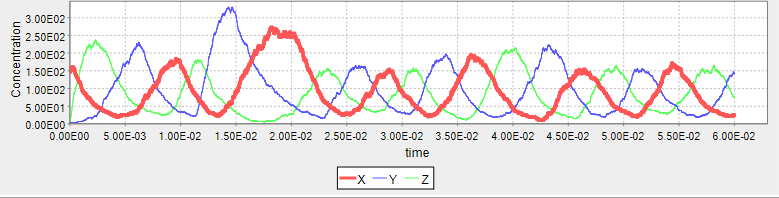
\includegraphics[width = 0.85\textwidth]{../images/nf_sim_interrupted_chart.png}
\caption{A plot of particle concentrations in the well-mixed repressilator model over time. Adding a significant number of \textvar{Y} particles to our simulation (the second blue peak) produces little ultimate disturbance to the concentrations of the three particles, which return to normal oscillations within a single cycle.}
\label{fig:nf_sim_interrupted_chart}
\end{figure}

Because of the spike in the concentration of \textvar{Y}, the reaction $\textvar{Y} + \textvar{Z} \rightarrow \textvar{Y}$ suppresses the concentration of \textvar{Z} for longer than usual, and so the concentration of \textvar{X} is free to increase for longer than normal. As a result, the next peak of \textvar{X} particles is higher than normal.

We might hypothesize that this process would continue, with a tall peak in the concentration of \textvar{Z}. However, the peak in the concentration of \textvar{Z} is no taller than normal, and the next peak shows a normal concentration of \textvar{X}. In other words, the system has very quickly absorbed the blow of an increase in concentration of \textvar{Y} and returned to normal within one cycle.

Even with a much larger jolt to the concentration of \textvar{Y}, the concentrations of the three particles return to normal oscillations very quickly (\autoref{fig:nf_sim_interrupted_chart_spike}).\\

\begin{figure}[h]
\centering
\mySfFamily
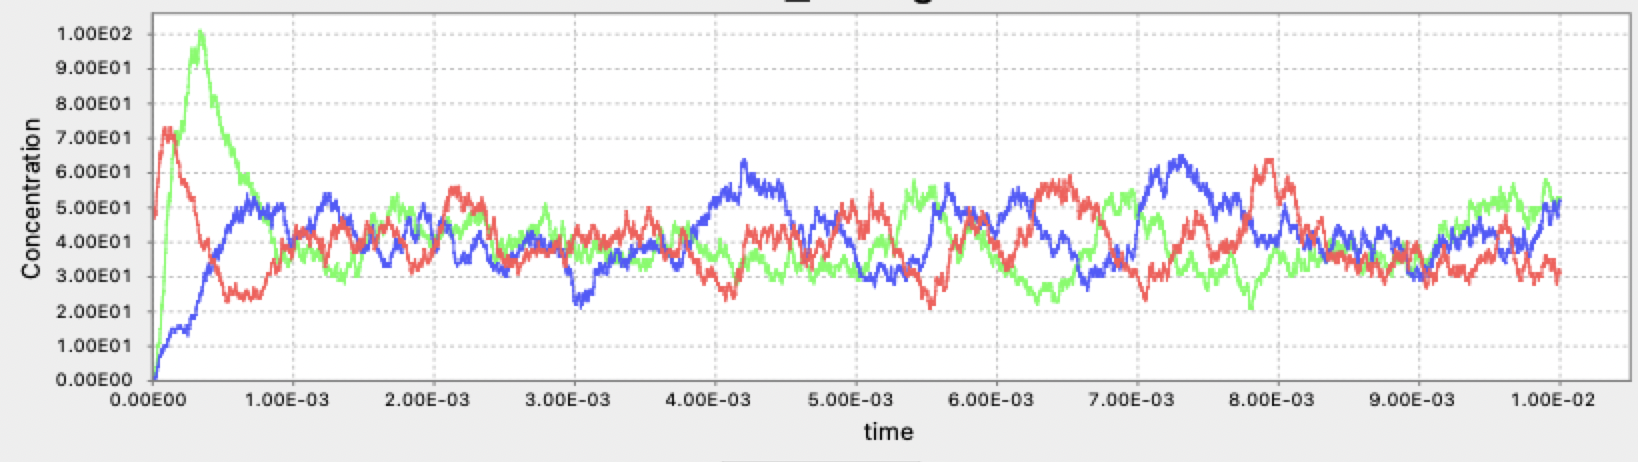
\includegraphics[width = 0.85\textwidth]{../images/nf_sim_interrupted_chart_spike.png}
\caption{A larger sudden increase in the concentration of \textvar{Y} particles than in \autoref{fig:nf_sim_interrupted_chart} still does not produce a substantive change in the system over time.}
\label{fig:nf_sim_interrupted_chart_spike}
\end{figure}

The repressilator is not the only network motif that leads to oscillations of particle concentrations, but robustness to disturbance is a shared feature of all these motifs. Furthermore, the repressilator is not the most robust oscillator that we can build. Researchers have shown that at least five components are typically needed to build a very robust oscillator, which may help explain why real oscillators tend to have more than three components.

%The repressilator's robustness implies a bigger picture moral of biological modeling. If an underlying biological system demonstrates robustness to change, then any model of that system should also be able to withstand this change. Conversely, in biology and in life, we should be skeptical of any non-robust model of a robust system.

In the next chapter, we will an even more involved biochemical process that is used by bacteria to cleverly (and robustly) explore their environment. In fact, replicating this system will require so many particles and so many reactions that we will need to rethink how we formulate our model.\\

\FloatBarrier
\section{Exercises}
\label{sec:exercises}
\phantomsection

\phantomsection
\subsection{Statistical validation}

\begin{exercise}[%
42 FFLs is significant.
]\end{exercise}

\begin{exercise}[%
Computing a p-value rigorously.
]\end{exercise}

\phantomsection
\subsection{Identifying feedforward loops and more complex motifs}

Recall that in the feedforward loop motif (illustrated in \autoref{fig:feed-forward_loop}), \textvar{X} is connected to \textvar{Y} and \textvar{Z}, and \textvar{X} is connected to \textvar{Z}.\\

\begin{exercise}[%
Count the number of feedforward loops in the transcription factor network for \textit{E.~coli}.
]\end{exercise}

There are eight types of feedforward loops based on the eight different ways in which we can label the edges in a feedforward motif; each edge can be labeled by a ``+'' or a ``-'' depending on whether that edge corresponds to activation or repression.\\

\begin{exercise}[%
Adapt your solution to the previous exercise to count the number of loops of each type present in the \textit{E.~coli} transcription factor network.
]\end{exercise}

\begin{exercise}[%
How many feedforward loops would you expect to see in a random network having the same number of nodes as the \textit{E.~coli} transcription factor network? How does this compare to your answers to the previous two questions?
]\end{exercise}

%More complex motifs may require more computational power to discover.
%
%[![image-center](../assets/images/600px/s_cerevisiae_tf_network.jpg){: .align-center}](../assets/images/s_cerevisiae_tf_network.jpg)
%Example of different motifs within the *S. Cerevisiae* network.[^scNetwork]
%{: style="text-align: center; font-size: medium;"}

%\begin{exercise}[%
%Can you modify our Jupyter Notebook for motif finding to identify circular loops of transcription factor regulation, such as the multi-component loop above?
%]\end{exercise}

\phantomsection
\subsection{Negative autoregulation}

\begin{exercise}[%
One way for the cell to apply stronger "brakes" to the simple regulation rate would be to simply increase the degradation rate, rather than implement negative autoregulation. From an evolutionary perspective, why do you think that the cell doesn't do this?
]\end{exercise}

Recall that we used the reaction reaction $X \rightarrow X + Y$ to represent simple regulation. We then built a model in a tutorial to run a mathematically controlled comparison between two simulated cells, one having only simple regulation, and the other also having negative autoregulation, which we represented using the reaction $Y + Y \rightarrow Y$.\tutorial[motifs/tutorial_nar_mathematically_controlled]\\

\begin{exercise}[%
Multiply the rate of $X \rightarrow X + Y$ by a factor of 100 in the cell having only simple regulation, and plot the concentration of $Y$ in both cells. By approximately what factor do you need to increase the rate of this reaction in the cell that includes negative autoregulation so that the steady-state concentration of $Y$ is the same in both cells?
]\end{exercise}


\phantomsection
\subsection{Positive autoregulation}

Although most of the autoregulating \textit{E.~coli} transcription factors exhibit negative autoregulation, 35 of these transcription factors autoregulate \textit{positively}, meaning that the transcription factor activates its own regulation. This network motif exists in processes in which the cell needs a cell to be produced at a slower, more precise rate than it would under normal activation. This occurs in some genes related to development, when gene expression must be carefully controlled.\\

\begin{exercise}[%
Design and implement a reaction-diffusion model to run a mathematically-controlled simulation comparing the positive autoregulation of a transcription factor \textvar{Y} against normal activation of \textvar{Y} by another transcription factor \textvar{X}. Plot the concentration of \textvar{Y} over time in the two circumstances.
]\end{exercise}


\phantomsection
\subsection{Implementing more network motifs}

\begin{exercise}[%
Use the NFSim tutorial implementing the repressilator as a basis to replicate the other network motif tutorials presented in this module.
]\end{exercise}
